\subsection{Vorgaben}
Es galt eine Architektur aufzubauen, die auf einer HalfEdge-Datenstruktur basiert. Das heißt insbesondere:
\begin{itemize}
\item Jeder Punkt kennt genau \textit{eine} seiner ausgehenden und \textit{keine} seiner eingehenden Kanten.
\item Jede Kante kennt nur ihren Ausgangspunkt, ihre Gegenkante, ihre nachfolgende Kante und die Fläche, an der sie liegt.
\item Jede Fläche kennt genau \textit{eine} ihrer umschließenden Kanten. 
\item Bei einem zusammenhängenden Mesh ist jeder Punkt von jedem anderen über die Kanten erreichbar.
\item Kanten, die am Rand des Meshes liegen, kennen eine Fläche, die man als ``Hole`` bezeichnet.
\end{itemize}
In den folgenden Abschnitten wird die erstellte Architektur dargestellt und kurz erklärt.

\subsection{Architektur}
Die Architektur des Projektes teilt sich im wesentlichen in ein Model- und ein View-Paket. 
Während das Model eine etwas erweiterte HalfEdge-Struktur bereitstellt, ist das View-Paket im wesentlichen für die Anzeige zuständig. 

Im folgenden soll zuerst das Model-Paket und anschlie\ss{}end das View-Paket vorgestellt werden.

\subsubsection{Model}
\begin{figure}[htbp]
\centering
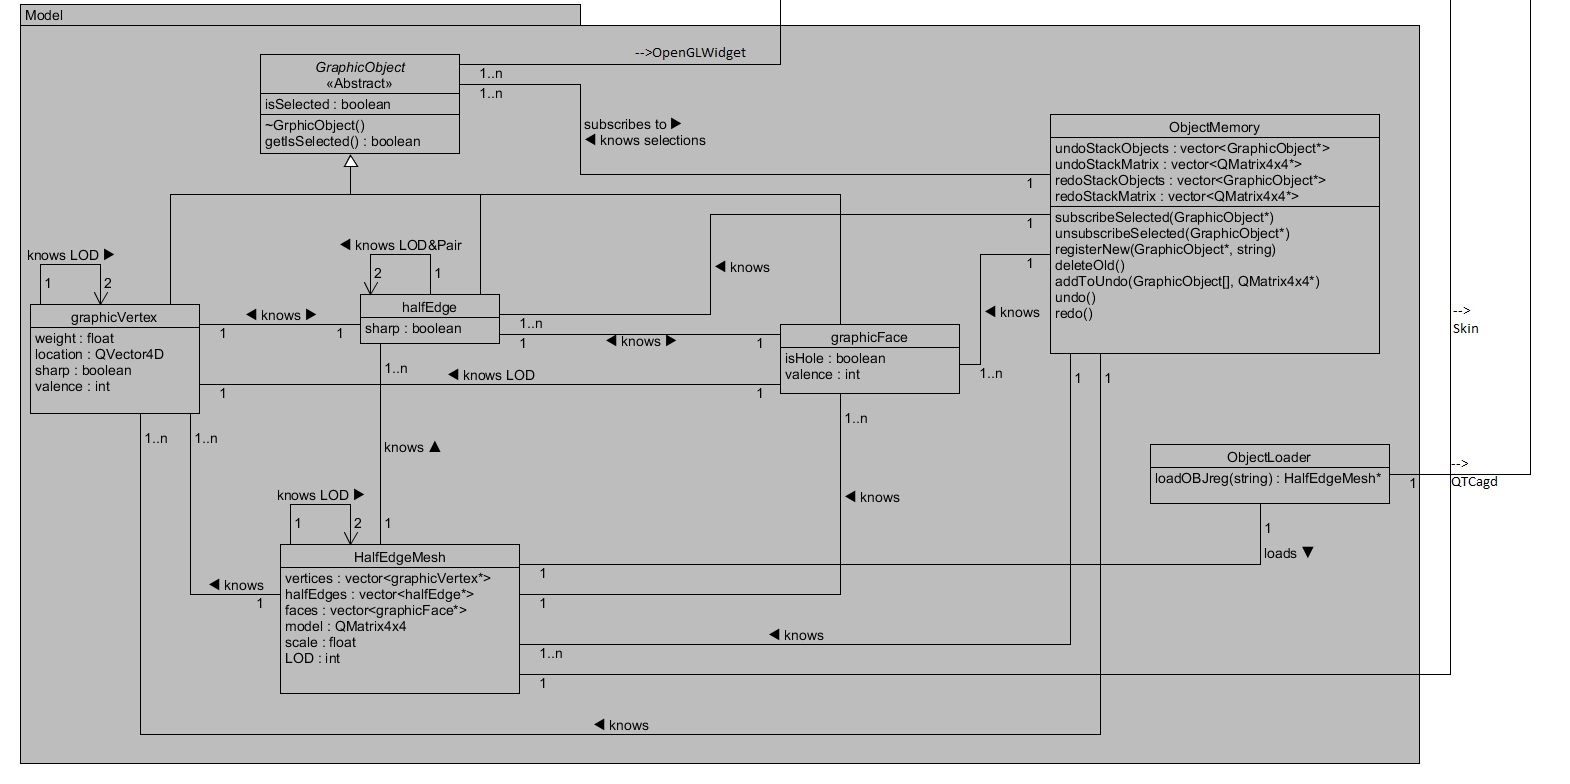
\includegraphics[angle=90,scale=0.5]{content/pictures/architekturModel.png}
\caption{Model-Paket der Architektur}
\label{fig:model}
\end{figure}

Wie bereits erwähnt stellt das Model in Abb.~\ref{fig:model} unter anderem die HalfEdge-Struktur bereit. 
Hierzu dienen die Strukturen graphicVertex, halfEdge und graphicFace, welche alle von der abstrakten GraphicObject-Klasse erben. 
Dies erleichtert später die Verknüpfung der verschiedenen Level of Detail (LOD) nach Ausführungen von Unterteilungsalgorithmen. 
Zur einfacheren Datenhaltung werden die genannten Strukturen als HalfEdgeMesh-Klasse gespeichert, die alle Punkte, Kanten und Flächen eines Objektes enthält. 
Des Weiteren kennt das Mesh sein LOD. 
Die genannten Objekte werden über die ObjectLoader-Klasse geladen.\\

Die ObjectMemory-Klasse ist zurzeit noch ungenutzt. 
Mit Verweis auf Kapitel~\ref{chap:Ausblick} sollte an dieser Stelle z.B. eine Undo-Redo-Funktion realisiert werden. 
Dies wurde aufgrund von Zeitmangel jedoch nicht umgesetzt.

\subsubsection{View}
\begin{figure}[htbp]
\centering
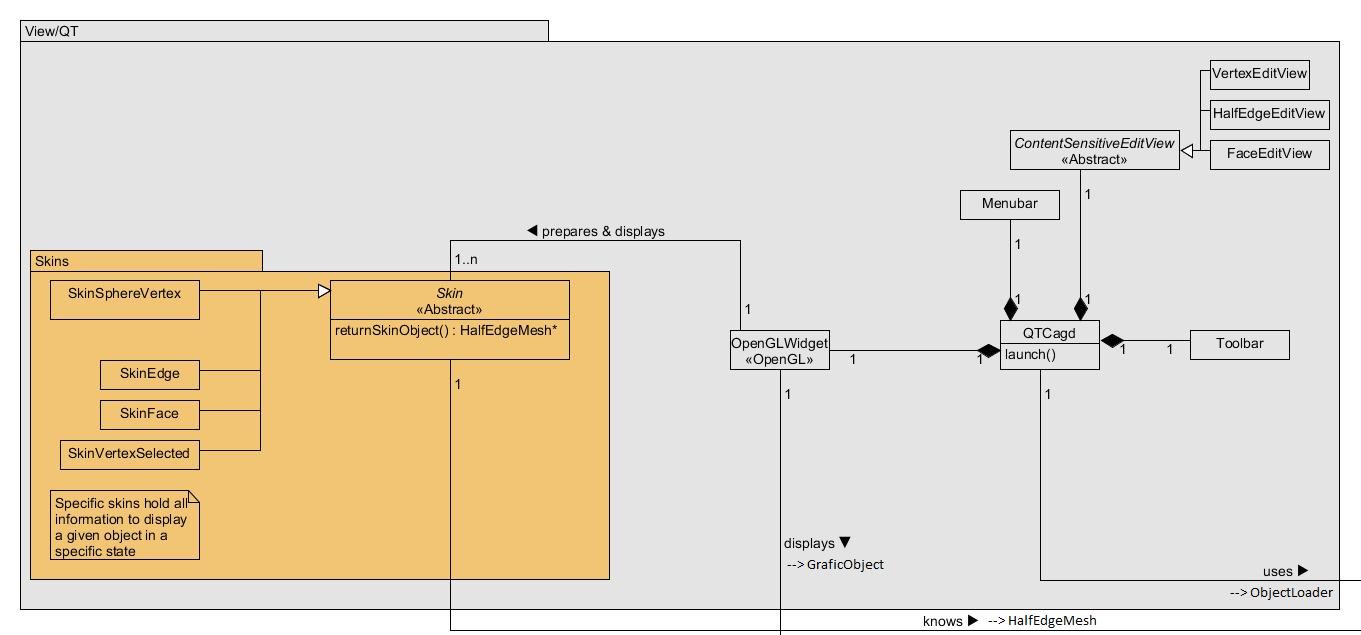
\includegraphics[angle=90,scale=0.6]{content/pictures/architekturView.png}
\caption{View-Paket der Architektur}
\label{fig:view}
\end{figure}

Um den Aufwand für UI-Programmierung zu reduzieren, haben wir uns des QT-Frameworks bedient. 
Dementsprechend besteht die View zum grö\ss{}ten Teil aus externen QT-Abhängigkeiten. 
Das Hauptfenster der Anwendung wird in QTCagd realisiert, welche eine mit dem QT-Designer erstellte QTCagd.ui einbindet und anzeigt (siehe Abb.~\ref{fig:view}).
Des Weiteren werden dort entsprechende Signale für UI-Eingaben und Auswahlen gesendet.

Das OpenGLWidget hingegen ist ein Teil des Hauptfensters und kümmert sich um sämtliche OpenGL-spezifischen Anzeigen und Operationen.
Dies umfasst z.B. das Anzeigen von Vertices, Edges und Faces. 

Das Skin-Paket umfasst Objekte, die zum Anzeigen der internen GraficObjects genutzt werden. 
So existiert z.B ein Sphere-Model, das genutzt wird, um dem Nutzer die Auswahl von Vertices zu erleichtern. 
Der ContextSensitiveEditView ist das Menü auf der rechten Seite in Abb.~\ref{fig:ui}. Dieses Menü ändert sich basierend auf der momentanen Auswahl.

\begin{figure}[htbp]
\centering
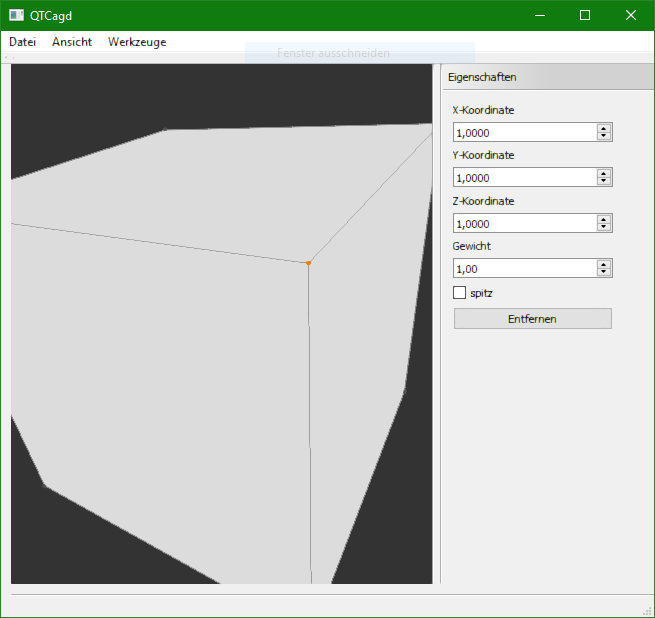
\includegraphics[scale=0.7]{content/pictures/cadgWindow.PNG}
\caption{UI der Anwendung}
\label{fig:ui}
\end{figure}